\lstset{language=[x64]Assembler}

Dalam pemograman, terdapat dua golongan bahasa pemograman bedasarkan sebagaimana
ia menyerupai bahasa mesin. Dalam hal ini golongan yang dimaksud adalah golongan
bahasa pemograman Low-Level (Tingkat Rendah) dan High-Level (Tingkat Tinggi).

Bahasa yang dikategorikan berada di level tingkat tinggi adalah bahasa yang
secara sintaks dan penggunaan lebih menyerupai bahasa yang digunakan seorang
manusia dan mudah dipahami oleh manusia, contohnya Python, Javascript, Ruby,
dan lain sebagainya. Untuk kategori satunya lagi, yaitu bahasa yang dikategorikan
berada di level rendah yaitu bahasa yang secara sintaks lebih sulit untuk dipahami,
dan memiliki fitur cenderung sangat dekat dengan sistem, contoh dari bahasa ini
adalah C, Pascal, ataupun Assembly.

Secara level, bahasa yang paling rendah adalah Assembly, karena ketika kita
meng-kompilasi atau lebih tepatnya assemble program Assembly instruksi-instruksi
yang tadi berbentuk sintaks akan dikonversi langsung kedalam bentuk Opcode.

Opcode ini adalah suatu nilai biner yang suatu prosessor akan terima sebagai instruksi,
dan dijalankan. Suatu opcode akan memiliki nilai-nilai seperti, jenis operasi yang
dikerjakan, dan jika terdapat data yang harus di proses dapat memiliki nilai seperti
di alamat memori atau register operasi dilakukan dan alamat ke tempat data
tersebut disimpan. Berikut adalah contoh dari bagaimana opcode terstruktur.

\begin{figure}[h]
    \centering
    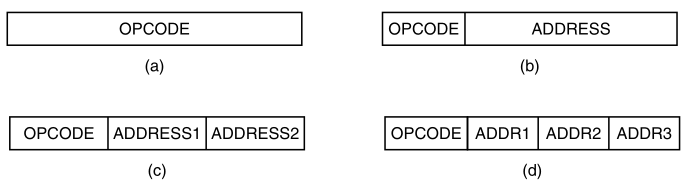
\includegraphics[scale=0.5]{OPCODEFORMAT}
    \caption{Format-format Opcode}
    \label{fig:OPCODEFORMAT}
\end{figure}

Dari program yang dicontohkan ini nantinya akan dapat dilihat opcode apa saja yang dihasilkan
dan kita dapat melihat bentuk suatu opcode secara langsung.

Bahasa pemograman yang digunakan adalah bahasa assembly untuk arsitektur x86. Alasan
dari digunakannya bahasa assembly di sini tidak bahasa lain seperti C, atau C++,
dikarenakan dalam menganalisis opcode yang dihasilkan, akan di jauh lebih sederhana
dibandingkan yang dapat dihasilkan oleh sebuah kompiler C ataupun C++ hingga jauh
lebih mudah untuk diteliti.

Untuk menjalankan program assembly ini diperlukan sebuah assembler dan juga linker,
yang saya gunakan adalah assembler x86 yang cukup populer yaitu NASM,
dan untuk linker program ld.

Fungsi dari sebuah assembler hampir serupa dengan sebuah kompiler, dalam arti
ia merubah suatu sintaks yang dimiliki suatu bahasa ke dalam instruksi yang
dapat dipahami oleh komputer. Namun sebuah assembler tersendiri tidak dapat membuat suatu
program dapat dijalankan oleh sistem, maka diperlukan linker yang akan menyatukan
instruksi-instruksi yang dihasilan assembler menjadi satu susunan program yang utuh.

Instruksi yang ditunjukan akan bedasarkan instruksi assembly dari arsitektur x86 32-bit,
berikut adalah contoh program yang akan melakukan serangkaian operasi aritmatika,
dan akan mengembalikan nilai akhir operasi-operasi tersebut di dalam \textit{exit-status} atau
nilai akhir ketika program tersebut berakhir.

Yang perlu dicatat juga tentang bahasa assembly, yaitu karena assembly berada di tingkat
yang cukup rendah, operasi yang ia lakukan akan register prosessor. Jadi dalam contoh berikut,
nama-nama seperti EAX, EbX, ECX, adalah nama atau identifier dari suatu register di processor.

Berikut adalah contoh program yang akan melakukan sejumlah operasi aritmatika, dan akan mengembalikan
nilai akhir dari operasi aritmatika tersebut sebagai exit code. Exit Code ini biasanya digunakan
untuk menyatakan berhasil atau tidak proses suatu program yang dijalankan.

\begin{lstlisting}
section .text

; nyatakan program mulai di label _start
global _start

_start:
  ; simpan nilai 3 di register 32 bit EBX
  mov EBX, 3

  ; simpan nilai 2 di register 32 bit ECX
  mov ECX, 2

  ; pertambahan nilai EBX dengan ECX
  ; ( EBX = ( 3 + 2 ) = 5 )
  add EBX, ECX

  ; pengurangan nilai EBX dengan ECX
  ; ( EBX = ( 5 - 2 ) = 3 )
  sub EBX, ECX

  ; perkalian nilai EBX dengan ECX
  ; ( EBX = (3 * 2) = 6)
  imul EBX, ECX

  ; pembagian nilai EBX dengan ECX
  ; ( EBX = (6 / 2) = 3)
  mov EAX, EBX
  idiv ECX
  mov EBX, EAX

  ; menentukan perintah sistem apa yang dijalankan saat interupt nanti
  ; perintah untuk hentikan program atau keluar
  ; direpresentasikan dengan angka 1
  mov EAX, 1

  ; sebabkan interupt,
  ; karena nilai EAX adalah 1 program akan berhenti atau keluar
  int 0x80

\end{lstlisting}
Dari program assembly yang dibuat diatas, terdapat beberapa operator aritmatika
yang dapat dilihat, yaitu penambahan, pengurangan, perkalian, serta pembagian.

Operasi-operasi tersebut akan dijelaskan sebagai berikut.

\begin{enumerate}

  \item \textbf{Operasi Penambahan}

    Di program sebelumnya operasi ini digambarkan dengan,

    \begin{lstlisting}
    add EBX, ECX
    \end{lstlisting}

    Operasi ini akan menambahkan nilai yang tersimpan di EBX dengan ECX.

    Jadi jika disana EBX sama dengan 3 dan ECX sama dengan 2. perhitungan
    yang terjadi adalah \textbf{EBX = (EBX + ECX)} atau \textbf{EBX = (3 + 2)},
    yang hasilnya adalah 2.

  \item \textbf{Operasi Pengurangan}

    Operasi pengurangan di program tersebut digambarkan dengan,

    \begin{lstlisting}
    sub EBX, ECX
    \end{lstlisting}

    Disini hampir sama dengan pertambahan sebelumnya, EBX bernilai 3 dan ECX bernilai 2,
    EBX akan dikurang dengan nilai ECX, dan nilai dari EBX adalah \textbf{EBX = (EBX - ECX)}
    atau bernilai 1.

  \item \textbf{Operasi Perkalian}

    Operasi pembagian di program tersebut digambarkan dengan,

    \begin{lstlisting}
    imul EBX, ECX
    \end{lstlisting}

    Sama seperti operasi sebelumnya operasi pembagian yang dilakukan disini sama saja,
    EBX dibagi dengan ECX, atau \textbf{EBX = (EBX * ECX)}.

  \item \textbf{Operasi Pembagian}

    \begin{lstlisting}
    idiv ECX
    \end{lstlisting}

    Operasi pembagian disini berbeda dengan yang lainnya karena, melibatkan register
    EAX. EAX sendiri adalah register accumulator. Dengan format instruksi terebut
    adalah \textbf{idiv N} secara perhitungan yang terjadi adalah \textbf{EAX = (EAX / N)}.

    oleh karena itu sebelum dijalan operasi tersebut niali EAX perlu dirubah ke nilai yang benar
    yaitu dengan perintah berikut.

    \begin{lstlisting}
    mov EAX, ECX
    \end{lstlisting}

    Operasi mov ini menyalin nilai ECX ke EAX. jadi perhitungan yang akan terjadi
    seakan-akan adalah EAX = (ECX / EBX).

    Dan setelah operasi selesai nilai yang berada di EAX harus di salin ke ke EBX agar
    dapat dilihat hasilnya.

    \begin{lstlisting}
      mov EBX, EAX
    \end{lstlisting}

\end{enumerate}

Hasil akhir dari program ini dapat dilihat dengan meng-assemble source code tersebut.
dan melihat apa nilai exit-code yang ia kembalikan.

Bedasarkan perhitungan, didalam program ini terjadi perhitungan berikut.

\textbf{(((( 3 + 2) - 2) * 2) / 2) = 3}

Mari dibuktikan.

\begin{figure}[h]
    \centering
    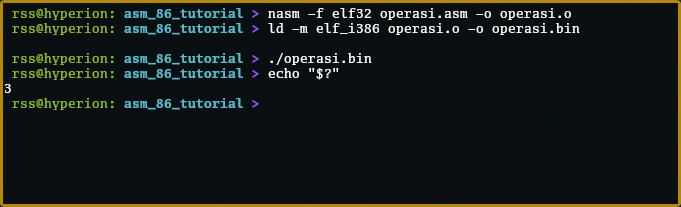
\includegraphics[scale=0.5]{HASILASM}
    \caption{Hasil dari program}
    \label{fig:HASILASM}
\end{figure}

Dapat terlihat, nilai exit code dari program tersebut benar maka program
tersebut berjalan dengan benar.

\newpage

Jika kita melihat object dump dari file executable yang dihasilkan, kita dapat
melihat opcode yang dihasilkan.

\begin{figure}[h]
    \centering
    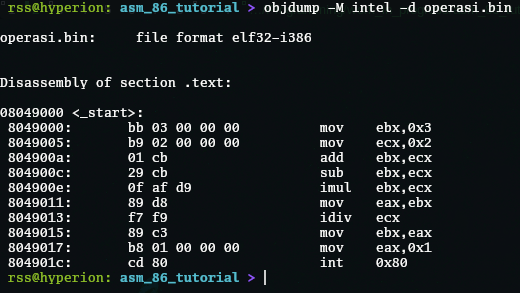
\includegraphics[scale=0.4]{HEXDUMPASM}
    \caption{Opcode dari program di format hexadecimal}
    \label{fig:HEXDUMPASM}
\end{figure}

Nilai opcode berada di kolom kedua, kita akan memastikan nilai opcode tersebut
benar bedasarkan instruksi assembly dari program sebelumnnya.
Kita dapat mengambil contoh dua opcode yang dihasilkan.

\begin{center}
\textbf{bb 03 00 00 00}

\textbf{b9 02 00 00 00}
\end{center}

Agar dapat membuktikan bahwa kedua opcode ini adalah instruksi untuk
memasukan angka ke suatu register (MOV), maka nilai ini perlu dibandingkan
dengan tabel opcode yang dimiliki oleh arsitektur ini. Data tabel opcode
ini biasanya dapat ditemui di buku manual suatu prosessor yang biasanya
akan diberikan atau disediakan oleh yang memproduksi prosessor tersebut.

\begin{figure}[h]
    \centering
    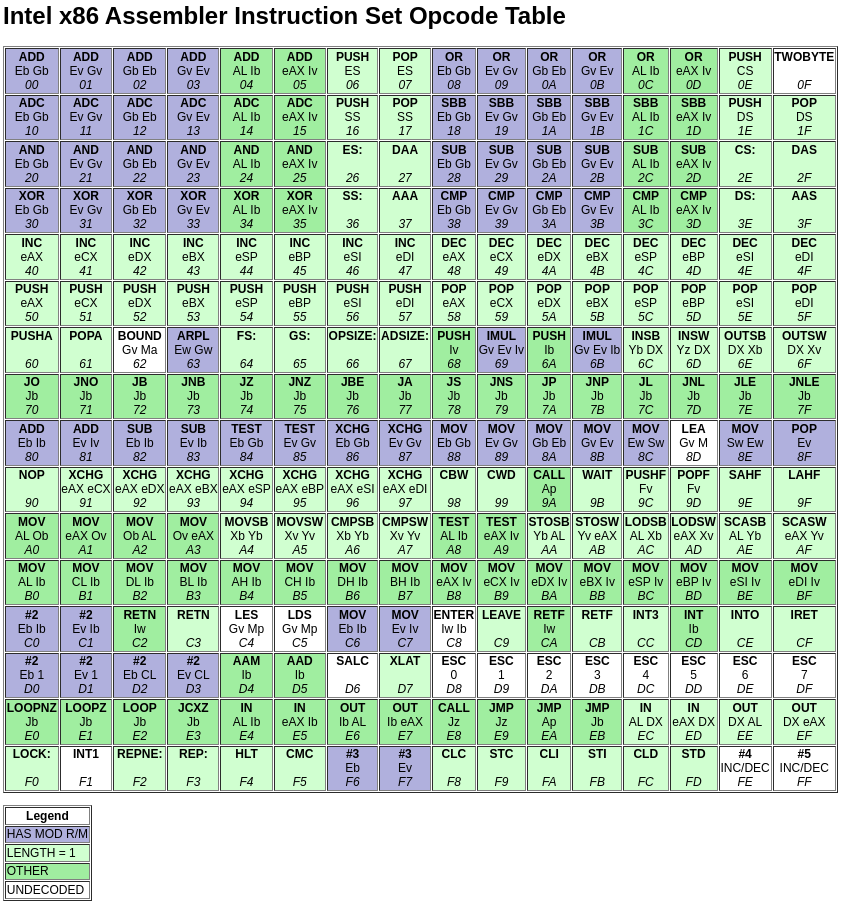
\includegraphics[scale=0.2]{INTELOPCODE}
    \caption{Tabel Opcode Aristektur x86 Intel}
    \label{fig:INTELOPCODE}
\end{figure}

Bedasarkan tabel di Gambar \ref{fig:INTELOPCODE} terdapat beberapa jenis operasi MOV,
dan MOV yang mengoperasikan register EBX adalah MOV yang bernilai hexadecimal BB, dan juga
MOV yang mengoperasikan register ECX bernilai hexadecimal B9.

Dari opcode yang diatas, juga terdapat nilai yang kita salin ke kedua register tersebut,
dan dapat dengan mudah dilihat dengan hexadecimal di kolom kedua opcode tersebut.

Maka dapat disimpulkan di kedua opcode tersebut, di kolom pertama menyimpan
tipe operasi yang dilakukan, dan di kolom selanjutnya menyimpan data yang digunakan.
